\chapter{The LHCb Detector}

The data used in this thesis originates from the LHCb Detector at the particle collider LHC or simulations thereof.
This detector is mainly focused on decays in which a bottom or a charm quark is involved. 
To accomplish this it has been build as a single arm forward-spectrometer, because the majority of $b$-/$c$-Hadron pairs are produced with velocities inside a cone around the beampipe.
An overview of the detector is shown in \autoref{fig:lhcb_detector}.
Its components are described briefly in this chapter.

\begin{figure}
    \centering
    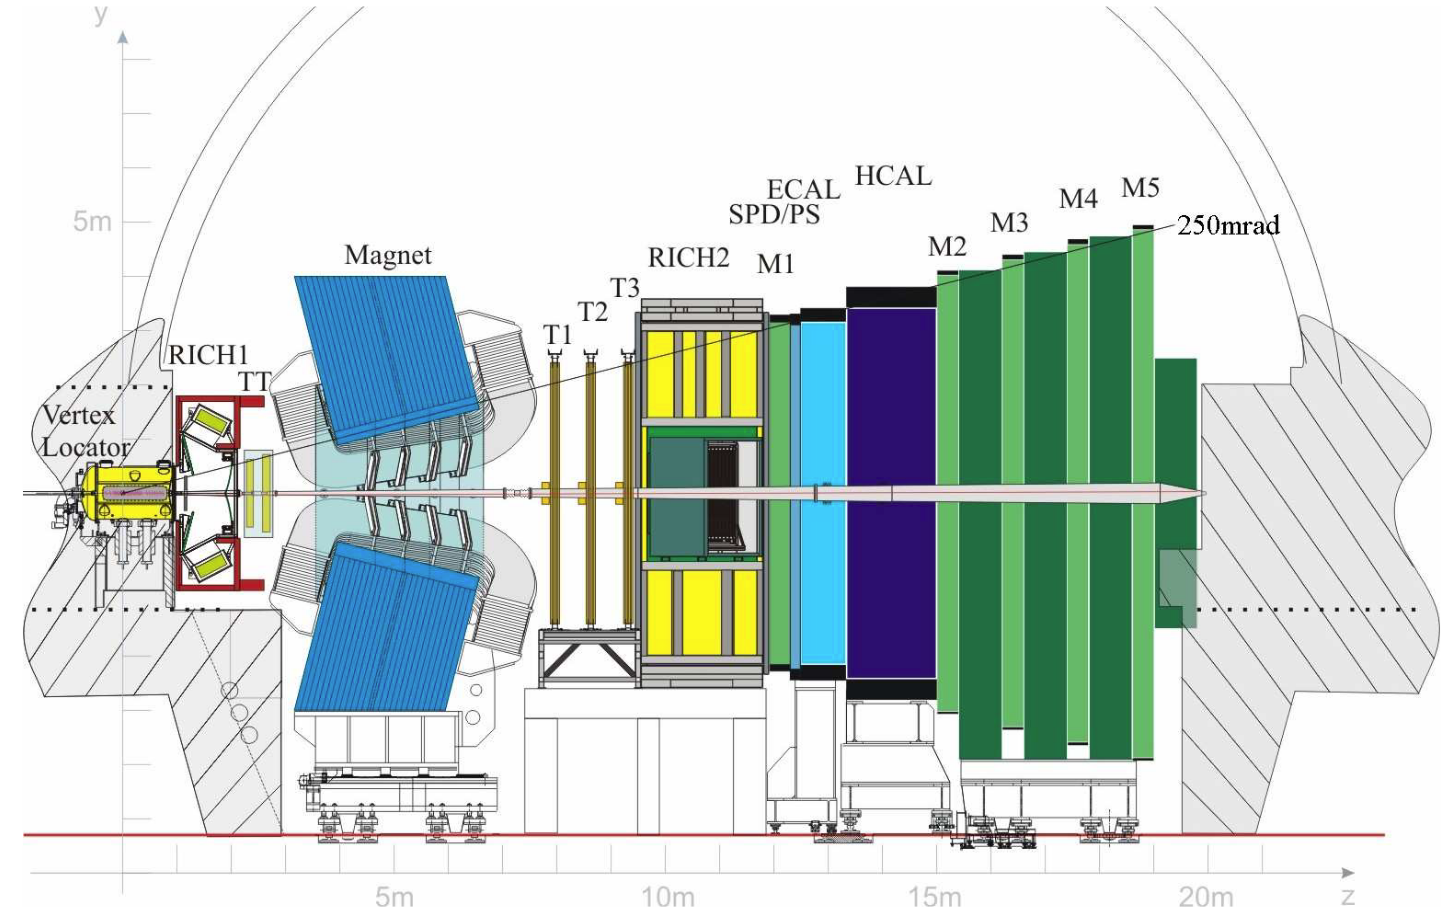
\includegraphics[width=\textwidth]{images/lhcb_detector.png}
    \caption{View of the LHCb detector. \cite{lhcb_detector}}
    \label{fig:lhcb_detector}
\end{figure}

The first detector element a particle traverses whis is produced at the collision point is the Vertex Locator (VELO). 
Here, the track of charged particles is measured using semi-conductor detectors. 
With this the point of the $pp$-collision (primary vertex) and the decay points can be reconstructed.

The next detector, the Ring Imaging Cherenkov detector 1 (RICH), measures the Cherenkov radiation produced by charged particles passing through a ...-Gel. 
The  

